\chapter{Implementing the Fault Detector}

After all the baseline foundations of deep learning and convolutional
neural networks have been derived, it is now time to apply these
methods to the problem of fault detection in the CLAS12 drift
chamber. Due to the CLAS12 productive environment heavily relying on
the JAVA programming language, all implementations are carried out
utilizing JAVA as well. The basis of the autonomous
fault detection system is formed by the deeplearning4j (DL4J)
library which is briefly described in the following section.

\section{The Deeplearning4j Library}

Deeplearning4j is an open-source deep learning library written for the
JAVA Virtual Machine (JVM). It is supported by the well known
AI-Startup Skymind and contains implementations of many algorithms
from the artificial intelligence domain, such as convolutional neural
networks, that will be used when implementing the fault detector.

To speed up the computations that have to be performed during the
training of deep convolutional architectures, DL4J relies on its own
numerical backend engine, ND4J, that contains C++ and Cuda
implementations of all required operations, most importantly matrix
multiplications. This way, deep neural networks can be trained on
big clusters containing multiple CPUs and GPUs, leveraging the huge
amounts of parallelism introduced by these computational
architectures.

Additionally, the DL4J library also provides useful mechanisms that
make monitoring the training process highly accessible, such as
Web-UIs which offer visual representations of the loss function as
well as the weight updates during training. Evaluating the trained
classifier is also not a difficult task, as DL4J provides
designated classes that are designed to compute all the relevant
metrics on the training dataset.\footnote{See
  \url{www.deeplearning4j.org} for more information.}

\section{Data Preparation}

Before the data can be fed into a convolutional neural network, a few
steps of preparation are necessary. Recall the heatmap plots of
different faults shown in section \ref{sec:faults}. The data that will
be presented to the network will be organized in the form of a \(6
\times 112\) array representing the activation level of each wire in a
superlayer, similar to the heatmaps. This way, the spatial structure
that is present within the data is preserved, which is essential when
working with CNNs, because as shown in section \ref{sec:convnets},
these architectures heavily depend on structural assumptions on the
input. Unlike in the case of images, the fault data will only consist
of a single channel, where every cell in the grid represents the
accumulated activations of a single wire, resulting in an input volume
of size \(6 \times 112 \times 1\).

Due to the fact that activation levels can vary drastically among
different regions, regions far away from the electron beam receiving
less particles passing by, the data has to be normalized in order to
compensate for these effects of disproportion. This is done by projecting
the activation values within each input on a numerical scale between 0
and 1, the lowest activation ending up at 0, the highest at 1. This
procedure will make it easier for the network to ignore the
differences in absolute activation levels and focus more on the local
fault patterns instead.

It should be noted that multiple ways of data normalization
were tested in the process of building the fault detector, e.g. computing
the standard score for every single wire in a superlayer.
This means adjusting all wire activations to show a mean of zero and a
variance of one. The described method did not yield strong results,
which is why among all the different approaches, also including
using the value of a sigmoid or a tanh function, the classic way of
normalization is used inside the fault detection system.

\section{The Fault Detection System}

When looking at the examples of various faults that can occur in the
drift chamber (see section \ref{sec:faults}), it becomes apparent that
there are usually multiple faults happening within a single
superlayer (see for instance Fig. \ref{fig:dead-connector}, where
there are a dead connector as well as multiple dead wires present in
the data). To account for these circumstances, multiple CNNs are
trained on the fault data, each individual CNN only specializing in
recognizing a single fault type (see section \ref{sec:faults} for a
summary of the different fault types), thus
resulting in a binary classifier for each fault. To obtain information
on the various faults present in a single input, each individual CNN
is presented with the corresponding data. In the next step, all the
individual responses are collected, resulting in a list of faults that
were recognized within the given superlayer. The network architecture
used is similar for each CNN that is part of the fault detector as
described in the following sections.

\subsection{Finding the Right Architecture}

One of the most challenging tasks when applying deep learning is to
find a set of suitable parameters that describe the network
architecture. These parameters, e.g. number of hidden layers, kernel
size of convolution layers, activation functions, learning rate,
\ldots are also refered to as \textit{hyperparameters}, because they
are set in advance and are not learned by the network during training.
In practice, the most common approach of finding the right
setup is to try many different architectures and configurations
and stick to those that work best.

During the process of designing the network that is used in the fault
detector, the simplest models, consisting of only a single convolution
layer followed by a pooling layer and fully connected layers, were
tested first. While working well with faults that are easily
recognizable, such as a dead channel, those models failed to capture
the more complex mechanisms of fault detection like dead wires. The
dead wire fault turned out to be the most complex of all because it
can basically appear everywhere, even next to each other. To cope with
these challenges, a deeper
architecture with six layers was used which was able to successfully
capture all the peculiarities associated with the various fault
types. This architecture, resulting from the process of testing
multiple combinations of hyperparameters, is presented in the next
section.

\subsection{Network Architecture and Configuration}

After the \(6 \times 112 \times 1\) input volume resulting from the
normalized activations of a superlayer, a convolution layer
is inserted as the first feature extractor of the network (see
Fig. \ref{fig:fault-architecture}), which
uses a kernel size of \(2 \times 3\) that accounts for the
unsymmetrical dimensions of the input. The total number of kernels
within this layer, i.e. the amount of features to look for, is set to
40 and a stride of 1 in each direction is used. The ReLU is applied
as an activation function to this layer. Another convolution layer is
inserted afterwards, this time using 30 kernels of size \(2 \times
2\), also setting stride to 1. The second convolution layer is
designed to search for higher level features by scanning the
activation maps of the first convolution layer.
Following these layers, a max-pooling layer is
employed with a filter size of \(2 \times 2\) and a stride of \(2
\times 2\) as well. This is done in order to compress the feature data
and contribute to the spatial invariance of the network (see section
\ref{sec:pooling}). Another convolution layer with 20
kernels of size \(2 \times 2\) is inserted next, scanning for even
higher level features in the downsampled output of the pooling
layer. Afterwards, a single fully
connected hidden layer with 100 hidden neurons is employed, utilizing
the ReLU activation function. The output layer consists of two
output neurons, one firing if the designated fault was detected, the
other firing if not. The softmax activation function is used on this
layer to make the outputs interpretable as probabilities. Overall, this
architecture results in a total of 113,182 parameters (weights and
biases) that have to be adjusted during training. An illustration of
the architecture can be found in Fig. \ref{fig:fault-architecture}.

Network initialization is performed using the Xavier
method (see section \ref{sec:xavier}), ensuring a weight distribution
that enhances network trainability. As for the optimization algorithm,
a slight variation of the traditional stochastic gradient
descent algorithm (see section \ref{sec:stochastic}) is employed,
called ADAM. The advantage of this algorithm is that it is able to
adjust the learning rate during training depending on the local
characteristics of the loss function by scaling the gradients based on
previous updates, resulting in a robust procedure for the training of
convolutional neural networks \cite{adam}. It's default learning rate
of 0.001 proved to be sufficient for the training task. The gradients
in each step of the updating process are computed using the
backpropagation algorithm (see section \ref{sec:backpropagation}).

\begin{figure}[h]
  \centering
  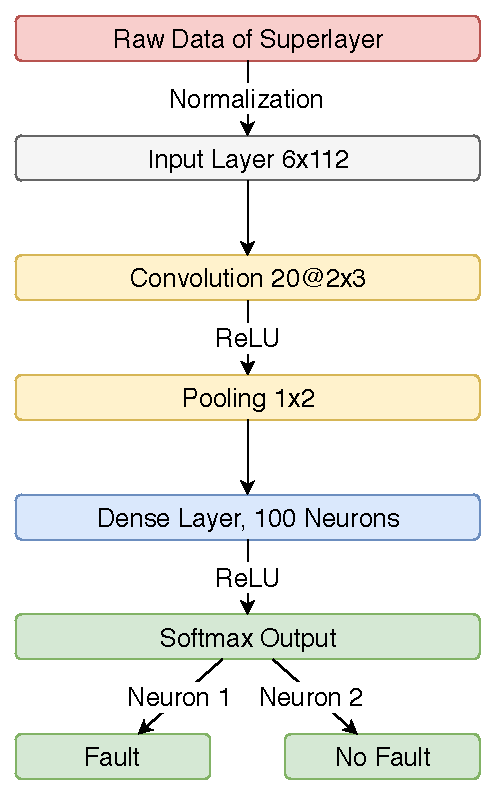
\includegraphics[width=.4\textwidth]{../figures/fault_architecture}
  \caption{The architecture of a single CNN in the fault detector that
  is trained to identify a unique fault type.}
  \label{fig:fault-architecture}
\end{figure}

\section{Training the Fault Detector}

In order to train the fault detector as a whole, every single binary
CNN was trained in isolation on a collection containing 100,000
positive and negative examples of the fault type that it is
supposed to detect. The data used during training was
generated by a simulation suite that works on real fault-free heatmaps
and inserts random combinations of faults which are then labeled in
accordance and fed into the network. In order to avoid overfitting
(see section \ref{sec:classification-architecture}), the wire activations
were randomly perturbed by the simulation suite during training,
ensuring that every example the classifier was presented with was
unique.

In the course of training the classifiers, the simulation suite had to
be adjusted multiple times to better capture all the various
characteristics of real fault data. At first, faults were only
inserted on completely randomized background signals which lead to
poor validation results on real data examples. After the simulation
suite was upgraded to work with background signals collected from real
experimental runs, performance on real data improved
significantly. Although the collected background signals
showed big differences in terms of activation patterns, which is due to
the fact that they were taken from different superlayers across
different regions, it turned out
that this circumstance did not harm the generalization ability of the
classifiers, as a single classifier dealing with all the different
background signals proved to be just as effective as multiple
classifiers, each specializing in a designated superlayer's background
signal.

The learning curve that plots the value of the loss function against
the first 5,000 training examples of the dead pin classifier, as
illustrated by the DL4J Web-UI, can be seen in
Fig. \ref{fig:learning-curve}. It strikes the eye that the
optimization algorithm seems to step through
rough terrain in the parameter space, as there are multiple spikes
occuring before convergence finally sets in. This is most likely due
to the fact that a batch size (see section \ref{sec:stochastic}) of
one was used during optimization, conciously inducing the spikes to
add more variation to the optimization process, increasing
the likelihood that a minimum will eventually be found. It should be
noted that bigger batch sizes of more than 20 examples were tested as
well, resulting in stagnation of the optimization procedure and not
leading to convergence. For this problem, it turned out, more noise
was helpful during training.

\begin{figure}[h]
  \centering
  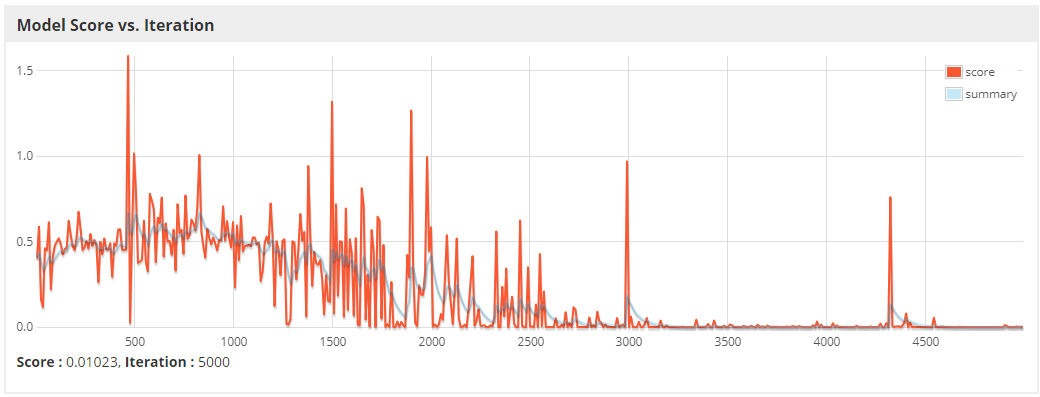
\includegraphics[width=\textwidth]{../figures/learning_curve}
  \caption{The DL4J Web-UI learning curve of the dead pin fault
    classifier for the first 5,000 examples shows many rough spikes
    but eventually leads to convergence.}
  \label{fig:learning-curve}
\end{figure}

\clearpage

\subsection{Training Results}

The training performance of every single binary classifier was
evaluated on 10,000 new randomly generated
examples using the common evaluation metrics as described in section
\ref{sec:classification-evaluation}. An overview of the results is
presented in the following paragraphs.

\paragraph{Dead Wire Classifier:}
\begin{itemize}
  \item Accuracy: 97.61\%
  \item Precision: 99.96\%
  \item Recall: 95.65\%
  \item F-Measure: 97.76\%
\end{itemize}
The confusion matrix of the dead wire classifier can be found in Table
\ref{tbl:confusion-deadwire}.
\begin{table}[h]
  \centering
  \renewcommand\theadfont{\bfseries}
  \begin{tabular}{|c|c|c|}
    \hline
    & \thead{Dead Wire\\(Predicted)} & \thead{No Dead Wire\\(Predicted)} \\
    \hline
    \thead{Dead Wire\\(Actual)} & 5212 & 237\\
    \hline
    \thead{No Dead Wire\\(Actual)} & 2 & 4549\\
    \hline
  \end{tabular}
  \caption{Confusion matrix of the dead wire classifier.}
  \label{tbl:confusion-deadwire}
\end{table}

\paragraph{Dead Pin Classifier:}
\begin{itemize}
  \item Accuracy: 99.95\%
  \item Precision: 99.92\%
  \item Recall: 99.98\%
  \item F-Measure: 99.95\%
\end{itemize}
The confusion matrix of the dead pin classifier can be found in Table
\ref{tbl:confusion-pin}.
\begin{table}[h]
  \centering
  \renewcommand\theadfont{\bfseries}
  \begin{tabular}{|c|c|c|}
    \hline
    & \thead{Dead Pin\\(Predicted)} & \thead{No Dead Pin\\(Predicted)} \\
    \hline
    \thead{Dead Pin\\(Actual)} & 4739 & 1\\
    \hline
    \thead{No Dead Pin\\(Actual)} & 4 & 5256\\
    \hline
  \end{tabular}
  \caption{Confusion matrix of the dead pin classifier.}
  \label{tbl:confusion-pin}
\end{table}

\paragraph{Dead Connector Classifier:}
\begin{itemize}
  \item Accuracy: 98.77\%
  \item Precision: 99.23\%
  \item Recall: 95.69\%
  \item F-Measure: 97.43\%
\end{itemize}
The confusion matrix of the dead connector classifier can be found in
Table \ref{tbl:confusion-connector}.
\begin{table}[h]
  \centering
  \renewcommand\theadfont{\bfseries}
  \begin{tabular}{|c|c|c|}
    \hline
    & \thead{Dead Connector\\(Predicted)} & \thead{No Dead Connector\\(Predicted)} \\
    \hline
    \thead{Dead Connector\\(Actual)} & 2334 & 105\\
    \hline
    \thead{No Dead Connector\\(Actual)} & 18 & 7543\\
    \hline
  \end{tabular}
  \caption{Confusion matrix of the dead connector classifier.}
  \label{tbl:confusion-connector}
\end{table}

\paragraph{Dead Fuse Classifier:}
\begin{itemize}
  \item Accuracy: 98.95\%
  \item Precision: 97.32\%
  \item Recall: 98.20\%
  \item F-Measure: 97.76\%
\end{itemize}
The confusion matrix of the dead fuse classifier can be found in Table
\ref{tbl:confusion-fuse}.
\begin{table}[h]
  \centering
  \renewcommand\theadfont{\bfseries}
  \begin{tabular}{|c|c|c|}
    \hline
    & \thead{Dead Fuse\\(Predicted)} & \thead{No Dead Fuse\\(Predicted)} \\
    \hline
    \thead{Dead Fuse\\(Actual)} & 2288 & 42\\
    \hline
    \thead{No Dead Fuse\\(Actual)} & 63 & 7607\\
    \hline
  \end{tabular}
  \caption{Confusion matrix of the dead fuse classifier.}
  \label{tbl:confusion-fuse}
\end{table}

\paragraph{Dead Channel Classifier:}
\begin{itemize}
  \item Accuracy: 99.11\%
  \item Precision: 98.84\%
  \item Recall: 98.64\%
  \item F-Measure: 98.74\%
\end{itemize}
The confusion matrix of the dead channel classifier can be found in Table
\ref{tbl:confusion-channel}.
\begin{table}[h]
  \centering
  \renewcommand\theadfont{\bfseries}
  \begin{tabular}{|c|c|c|}
    \hline
    & \thead{Dead Channel\\(Predicted)} & \thead{No Dead Channel\\(Predicted)} \\
    \hline
    \thead{Dead Channel\\(Actual)} & 3493 & 48\\
    \hline
    \thead{No Dead Channel\\(Actual)} & 41 & 6418\\
    \hline
  \end{tabular}
  \caption{Confusion matrix of the dead channel classifier.}
  \label{tbl:confusion-channel}
\end{table}

\paragraph{Hot Wire Classifier:}
\begin{itemize}
  \item Accuracy: 100.00\%
  \item Precision: 100.00\%
  \item Recall: 100.00\%
  \item F-Measure: 100.00\%
\end{itemize}
The confusion matrix of the hot wire classifier can be found in Table
\ref{tbl:confusion-hotwire}.
\begin{table}[h]
  \centering
  \renewcommand\theadfont{\bfseries}
  \begin{tabular}{|c|c|c|}
    \hline
    & \thead{Hot Wire\\(Predicted)} & \thead{No Hot Wire\\(Predicted)} \\
    \hline
    \thead{Hot Wire\\(Actual)} & 5532 & 0\\
    \hline
    \thead{No Hot Wire\\(Actual)} & 0 & 4468\\
    \hline
  \end{tabular}
  \caption{Confusion matrix of the hot wire classifier.}
  \label{tbl:confusion-hotwire}
\end{table}

\section{Validation on Real Data}

Overall, these results are looking rather promising. One has to keep in mind
however, that all the examples the classifiers were trained on have
been generated by a simulation suite. To prove, that the classifiers
are able to generalize beyond the simulations and successfully adapt
to real world data, some concrete examples are discussed in more
detail in the scope of this section, showing the strengths as well as
some weaknesses of the fault detection system.

\paragraph{Example 1 - A Pin Fault and Dead Wires:}

Fig. \ref{fig:pin-success} shows a superlayer that contains a dead pin
as well as some dead wires.  Both the dead wire classifier as well as
the dead pin classifier report with 100\% certainty that they detected
a fault. All the other classifiers are more than 99\% certain that
their designated fault type is not present within the
superlayer. This example illustrates that the model had no difficulty
in recognizing these clearly defined faults.

\begin{figure}
  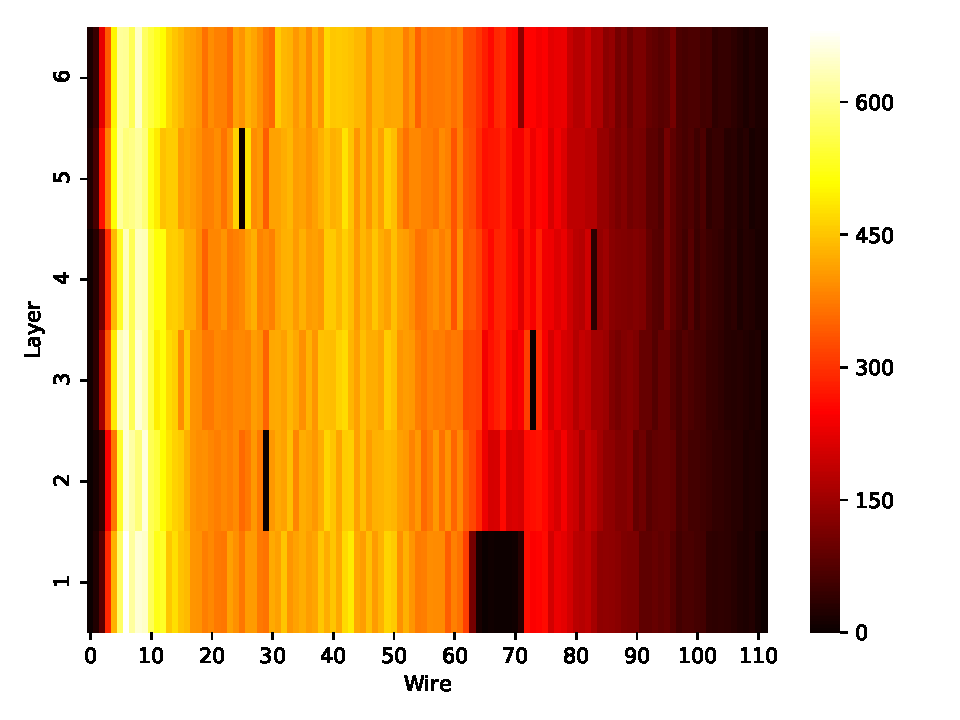
\includegraphics[width=\textwidth]{../figures/small_pin_success}
  \caption{A superlayer showing a faulty pin as well as some dead
    wires.}
  \label{fig:pin-success}
\end{figure}

\paragraph{Example 2 - A Dead Connector and Dead Wires:}

When presented with a dead connector as shown in
Fig. \ref{fig:connector-success}, the classifier succeeds spotting the
dead connector with 100\% certainty. The dead wires around that
connector are successfully detected with 100\% certainty as well. In
this example, there is a little more noise present around the dead
connector which turns out not to be a problem for the classifier.

\begin{figure}
  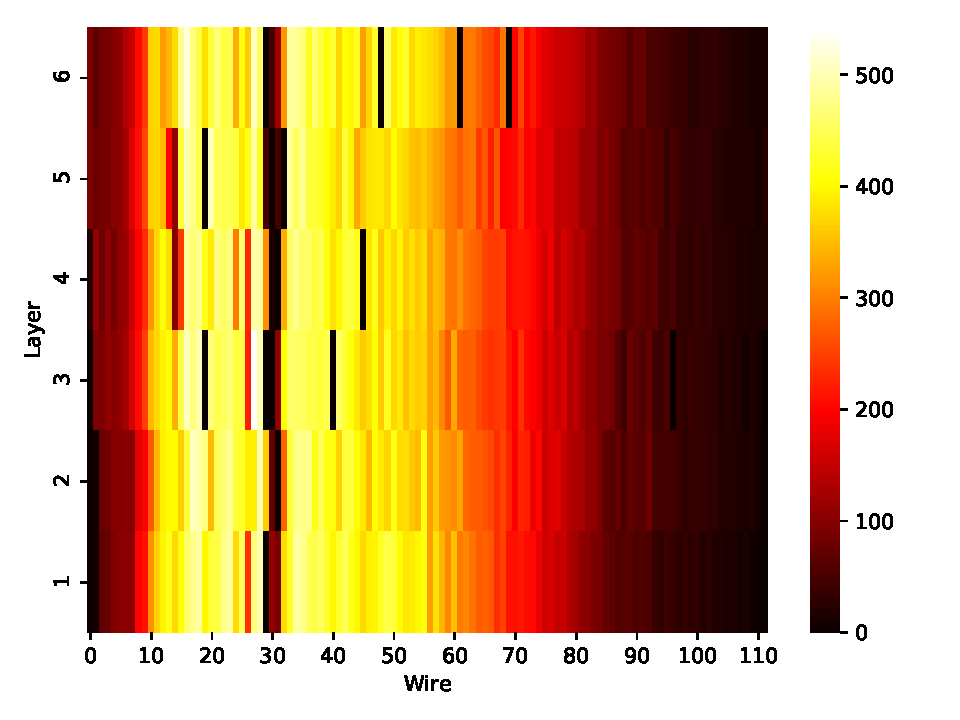
\includegraphics[width=\textwidth]{../figures/dead_connector_success}
  \caption{This superlayer contains a dead connector fault as well as
    some dead wire faults.}
  \label{fig:connector-success}
\end{figure}

\paragraph{Example 3 - A Blurred Dead Pin:}

When the fault is not as clearly defined as it was in previous
examples, the detector starts showing some signs of
difficulty. In Fig. \ref{fig:pin-failure}, we can see a dead pin that
does not display such a high contrast with respect to its environment.
The model struggles with this example, showing a certainty of over
99.99\% that no dead pin is present in the superlayer. The dead wire
that is also visible in this example was recognized with 100\%
certainty, not showing any problems.

This example illustrates that the classifier shows signs of weakness
when faults are blurry and not clearly defined, which is
also the case with other faults such as dead channels or dead
fuses. Whenever a component of a superlayer is not completely dead but
clearly faulty, the classifier struggles in recognizing the
fault. This problem could be remedied however, by presenting the
classifier with more blurry examples during training. It was decided
that this would best be accomplished by training the classifier on
real data examples that also include blurred faults. At the time of
writing, this data was not yet available, which is why solving this
problem will be part of future work.

\begin{figure}
  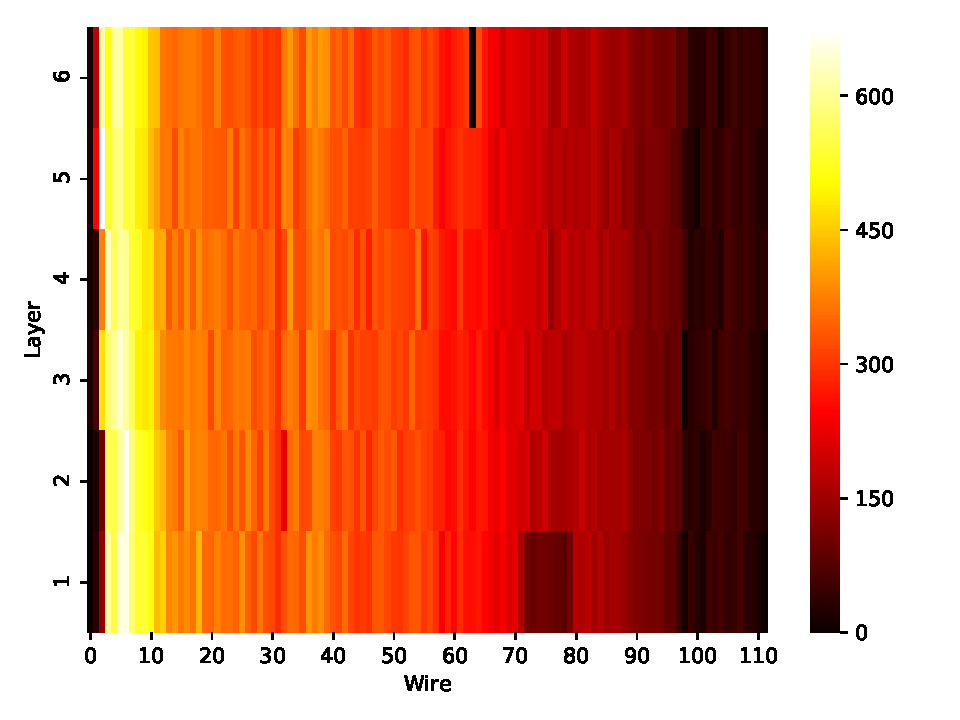
\includegraphics[width=\textwidth]{../figures/small_pin_fail}
  \caption{This superlayer shows a blurred example of a dead pin that
    caused problems in classification.}
  \label{fig:pin-failure}
\end{figure}

\clearpage

\paragraph{Example 4 - Two Dead Wires Next to Each Other:}

In Fig. \ref{fig:two-wires} we can see the interesting situation that
two dead wires are right next to each other. Despite this being a rare
occasion, the classifier was able to report with 93.29\% certainty
that it spotted a dead wire. The dead pin that is also present in this
example was recognized with 100\% certainty.

\begin{figure}
  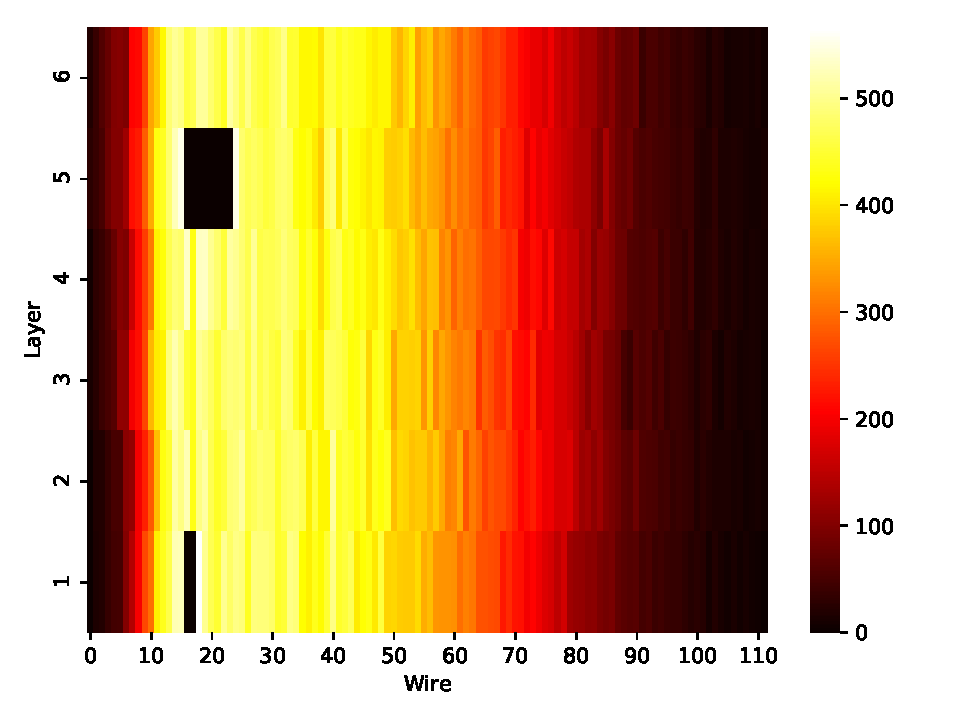
\includegraphics[width=\textwidth]{../figures/two_wires}
  \caption{Two dead wires next to each other in layer one.}
  \label{fig:two-wires}
\end{figure}
